\section{Гаммы? Импровизация в жестких рамках}
\label{ch:harmony:scales}

Мы уже разобрались с тем, что такое лад, тональность и гамма в разделе \ref{ch:harmony:lad}. Вкратце, гамма --- это последовательно сыгранные ступени лада, отложенного от <<базовой>> ноты (тоники). Или, например, гамма --- это последовательно сыгранные ступени тональности.

Зачем играть гаммы?
\begin{itemize}
    \item Гамма приятно звучит, никакого дискомфорта, так почему бы и не сыграть?
    \item Начинающим полезно играть гаммы, проговаривая входящие ноты вслух, чтобы лучше запомнить их положение на грифе гитары.
    \item Гаммы --- это неплохая тренировка для пальцев. Даже профи, знающие множество простеньких пьес, чтобы разыграться перед выступлением, не гнушаются гаммами.
    \item Так как гамма --- это конкретный вариант \emph{лада}, то в каком порядке не играй ноты гаммы --- будет МУЗЫКА. Расслабьтесь, комбинируйте, играйте с длительностью, акцентами, импровизируйте. В конце концов музыка должна приносить удовольствие даже на этапе обучения!
\end{itemize}

Итак, ноты нотами, а играть-то нужно ручками. Поэтому на первых этапах придется потратить время на то, чтобы соотнести ноты с постановкой и движениями рук. Для гитары вопрос нот сводится к постановке пальцев левой\footnote{Если левши внимательно читали примечания, то они знают, что автор надеется, что они знают, что делать} руки на грифе. 

\begin{Definition}[Аппликатура]
    \emph{Аппликатура}\footnote{От латинского applico --- прикладываю, прижимаю} --- порядок расположения и чередования пальцев при игре на музыкальном инструменте.
\end{Definition}

Чтобы задать аппликатуру, гитаристы обычно пользуются изображением кусочка грифа, на котором точками отмечены места прижатия струн, а при необходимости возле точки указан и номер пальца левой руки. Такой рисунок называется \emph{аппликатурным боксом}. Пальцы левой руки принято нумеровать слеюдующим образом:
\begin{itemize}
    \item указательный --- 1;
    \item средний --- 2;
    \item безымянный --- 3;
    \item мизинец --- 4.
\end{itemize}

Большой палец на левой руке не нумеруется, ибо находится с тыльной стороны грифа и оказывает моральную поддержку остальным пальчикам, имеющим дело со струнами.

Нам уже известно, что только диатонических ладов (включающих мажор и минор) семь штук, пентатоник --- пять. Так что имеется большой выбор в каком ладу поиграть. А о тональностях и говорить нечего --- смело умножайте количество ладов на 12!

Давайте ограничимся примерами на гамме ДО-мажор. При желании с остальными можно разобраться по аналогии. Не надо думать, что нужно уметь играть гаммы во всех ладах и тональностях. Вы же не робот! А если робот, то вот неплохое чтиво\footnote{Признанным специалистом в области гамм является Андреас Сеговия, чьи гаммы играет не первое поколение классических гитаристов. Открыв его книжку \cite{bib:segovia:Scales} можно увидеть 9 страниц нотной записи гамм (с аппликатурными пометками) во всех тональностях мажорного и минорного ладов. Эта книжка --- справочник, методичка, её с ужасом открывает на нужной странице бедный ученик музыкальной школы, терзает заданную учителем гамму, и с ужасом закрывает обратно, чтобы навсегда о ней забыть. Через несколько десятков лет, ставший профессионалом ученик, возможно и откроет книжку Сеговии, чтобы подглядеть как ставил на струны свои гениальные пальцы маэстро. Из любопытства. И только потому, что сам ужасно много знает}: \cite{bib:segovia:Scales} справочник от гениального гитариста и педагога Андреаса Сеговии.

\begin{Example}[Гамма ДО-мажор на одной струне]
    \label{ex:harmony:scales:d:maj}
    
    Нота ДО находится на первом ладу второй струны. Последовательно зажимайте на второй струне указательным пальцем левой руки лады 1-й, 3, 5, 6, 8, 10, 12, 13 и одновременно с этим защипывайте правой рукой вторую струну. Прозвучит гамма ДО-мажор. Одна октава от ДО первой октавы до ноты ДО второй октавы. 
    
    При этом мы прошлись вдоль всего грифа, сдвигая руку по струне.
    
    Выводы:
    \begin{itemize}
        \item неудобно: сдвиг руки вдоль по грифу --- слижком грубое движение, о быстрой игре можно забыть;
        \item неэкономно: музыка --- не спорт, но если так руками махать, то понадобится допинг;
        \item непрактично: одни и те же ноты есть в разных местах на грифе.
    \end{itemize}
\end{Example}

Два экономных варианта исполнения гаммы ДО-мажор приведены на рисунке \ref{fig:harmony:scales:c:dur1}. Левая рука двигается только поперек грифа и каждый палец отвечает только за свой лад. Аппликатура слева --- гамма в одну октаву, а спрва --- двухоктавная гамма. В серых кружочках --- местах прижатия струны, написано латинское обозначение ноты, а не номер пальца (так как пальцы вдоль грифа не сдвигаются, то в этом нет необходимости). Стрелочками показан порядок постановки пальцев на струны при игре <<по восходящей>> --- дойдя до конца, играйте в обратной последовательности.

\begin{figure}[!ht]
    \centering
    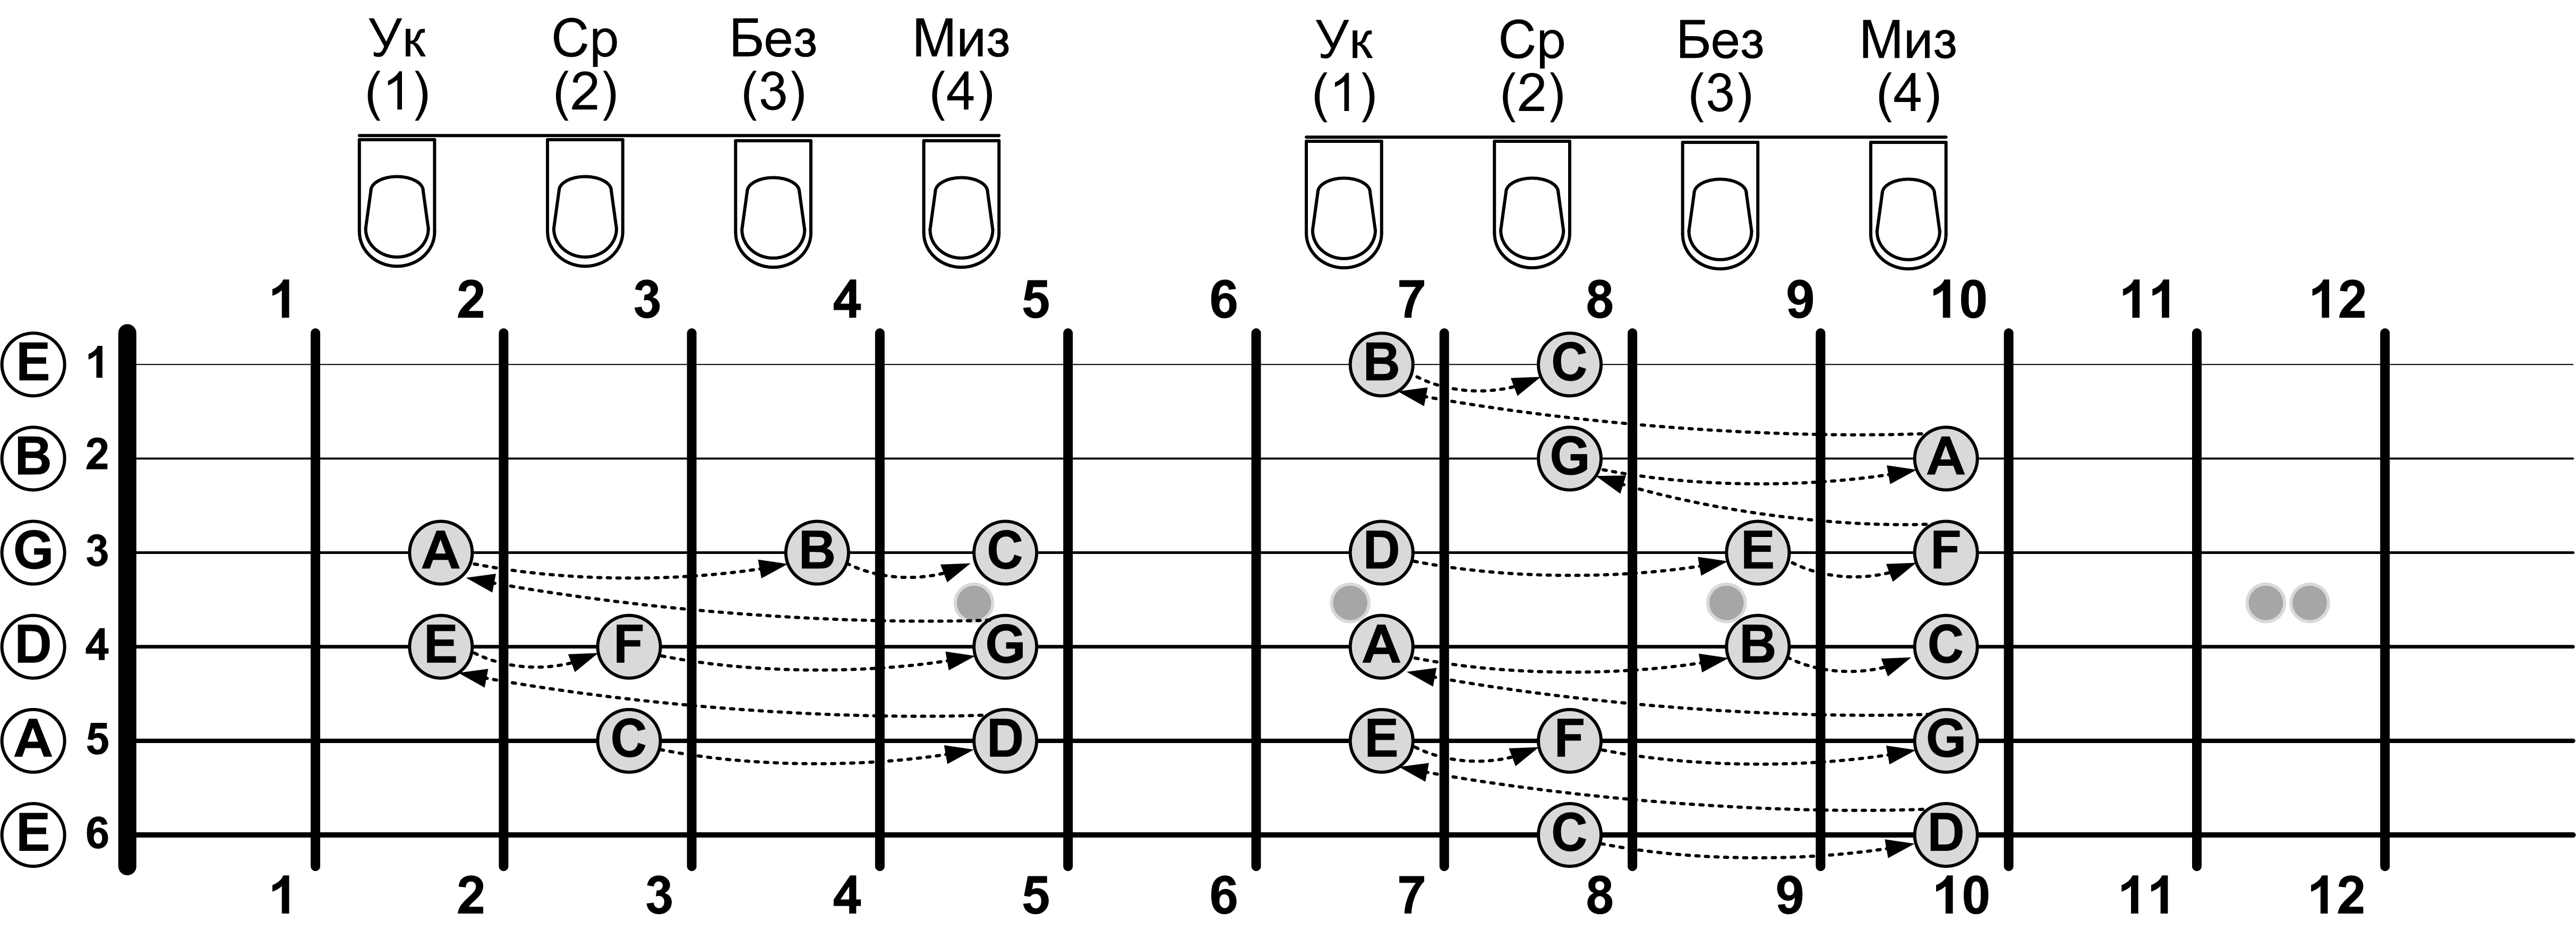
\includegraphics[width=\textwidth]{fig/intervals/c-dur-csale-1} 
    \caption{Два варианта аппликатур гаммы ДО-мажор}\label{fig:harmony:scales:c:dur1}
\end{figure} 

Стоит отметить, что во время испольнения не следует снимать (поднимать над грифом) раньше времени пальцы, которые можно оставить. Хотя новичку, пока нет независимости в пальцах левой руки, это будет трудно и этим правилом можно пренебречь.

Если внимательно поискать на грифе места, где еще можно сыграть гамму ДО-мажор не растопыривая пальцы слишком широко и не смещаясь вдоль грифа, то можно найти вариант, представленный на рисунке \ref{fig:harmony:scales:c:dur2}.

\begin{figure}[!ht]
    \centering
    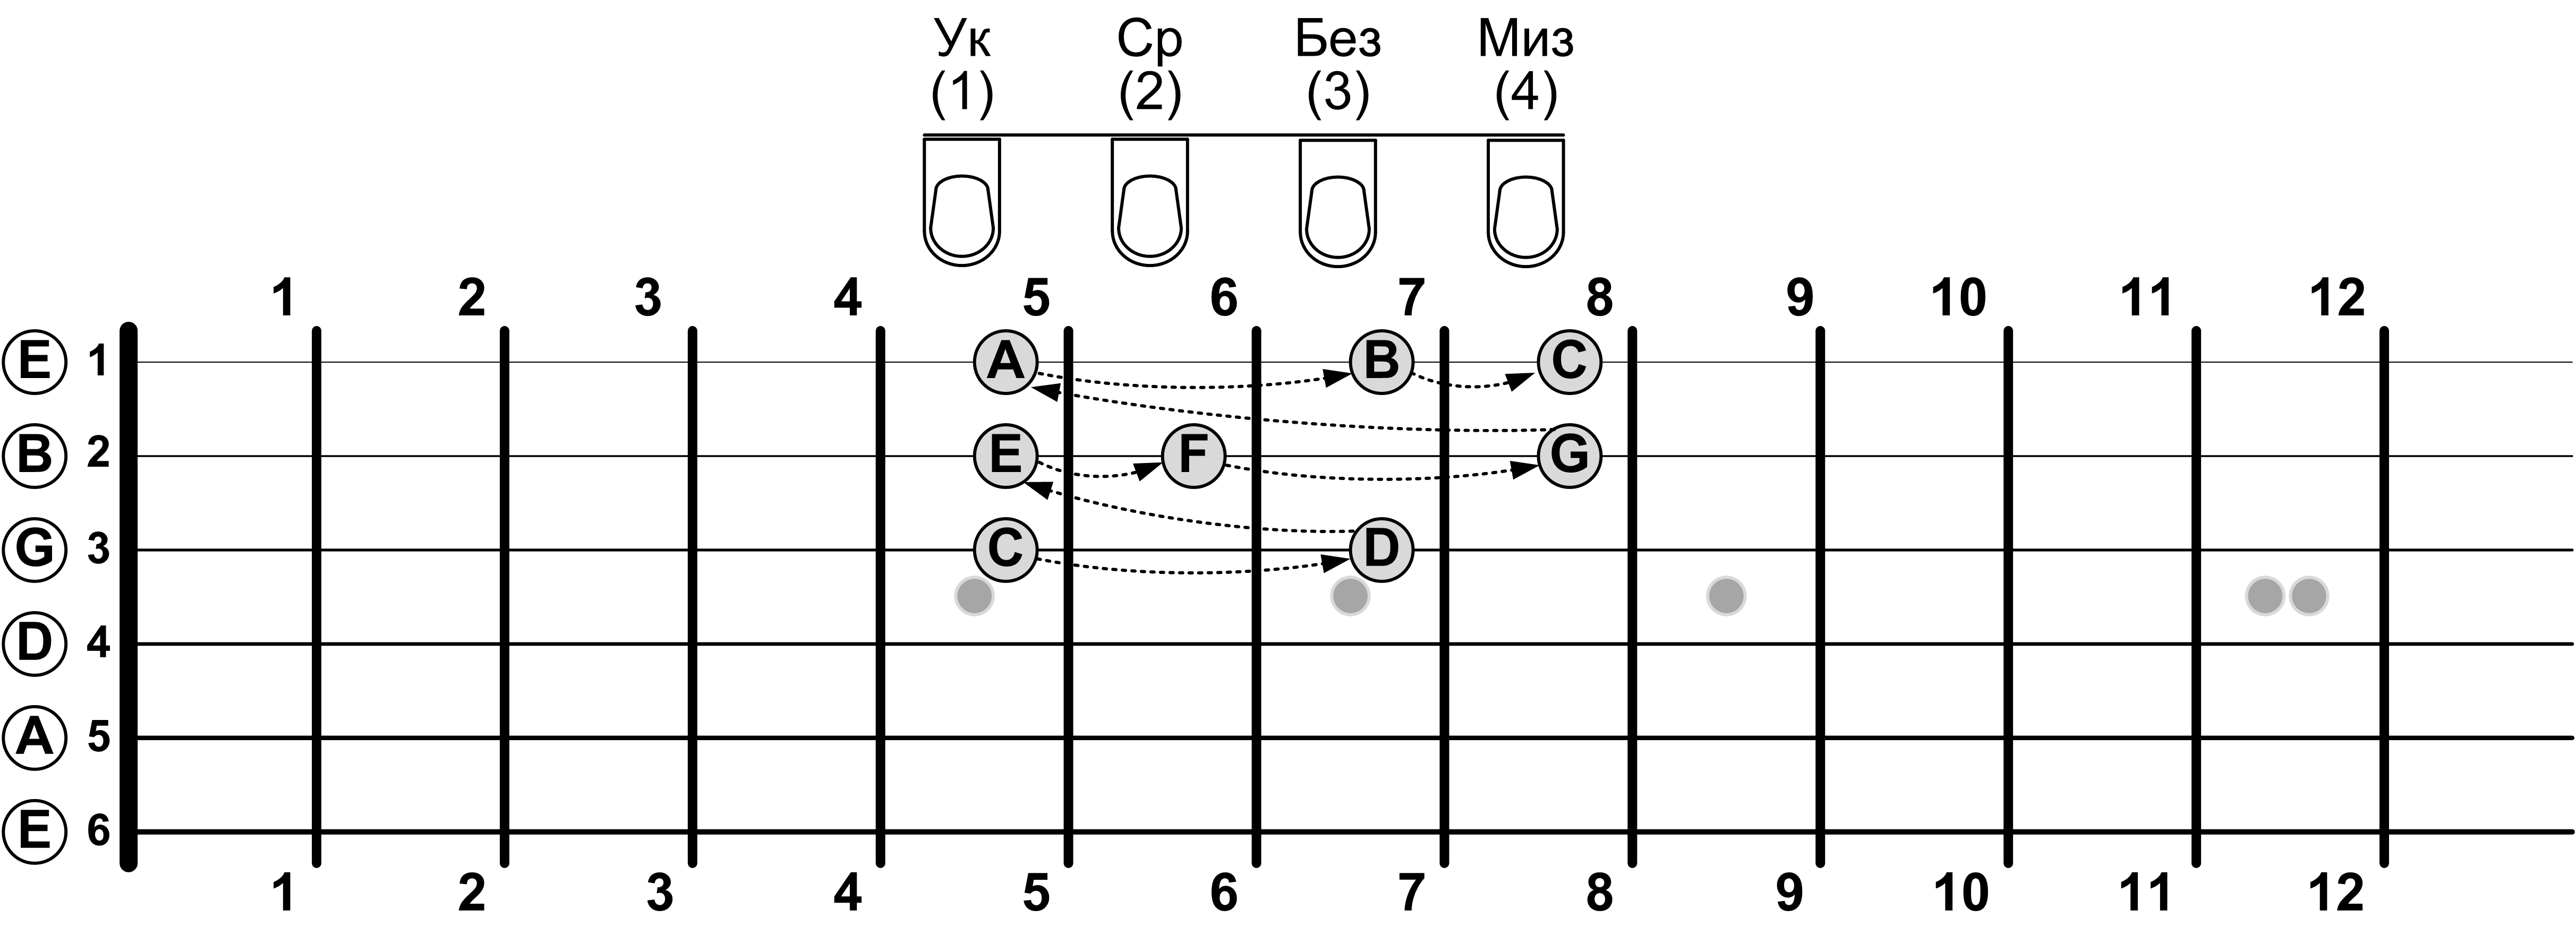
\includegraphics[width=\textwidth]{fig/intervals/c-dur-csale-2} 
    \caption{Аппликатура однооктавной гаммы ДО-мажор}\label{fig:harmony:scales:c:dur2}
\end{figure} 

Но смещаться по грифу на практике все-таки придется. Вариант двухоктавной гаммы ДО-мажор от Андреаса Сеговии приведен на рисунке \ref{fig:harmony:scales:c:dur:segovia}. В кружках, как и положено, написаны номера пальцев левой руки. Фрагменты этого аппликатурного шаблона вы можете увидеть по-отдельности на рисунках \ref{fig:harmony:scales:c:dur1} и \ref{fig:harmony:scales:c:dur2}. По третьей струне придется испытать неудобства: после того, как 3-м пальцем на 4-м ладу сыграна нота СИ(B), нужно быстро и точно переставить (или <<съехать>>, если струна гладкая) кисть так, чтобы указательный палец встал на 5-й лад (ноту ДО(C)).

\begin{figure}[!ht]
    \centering
    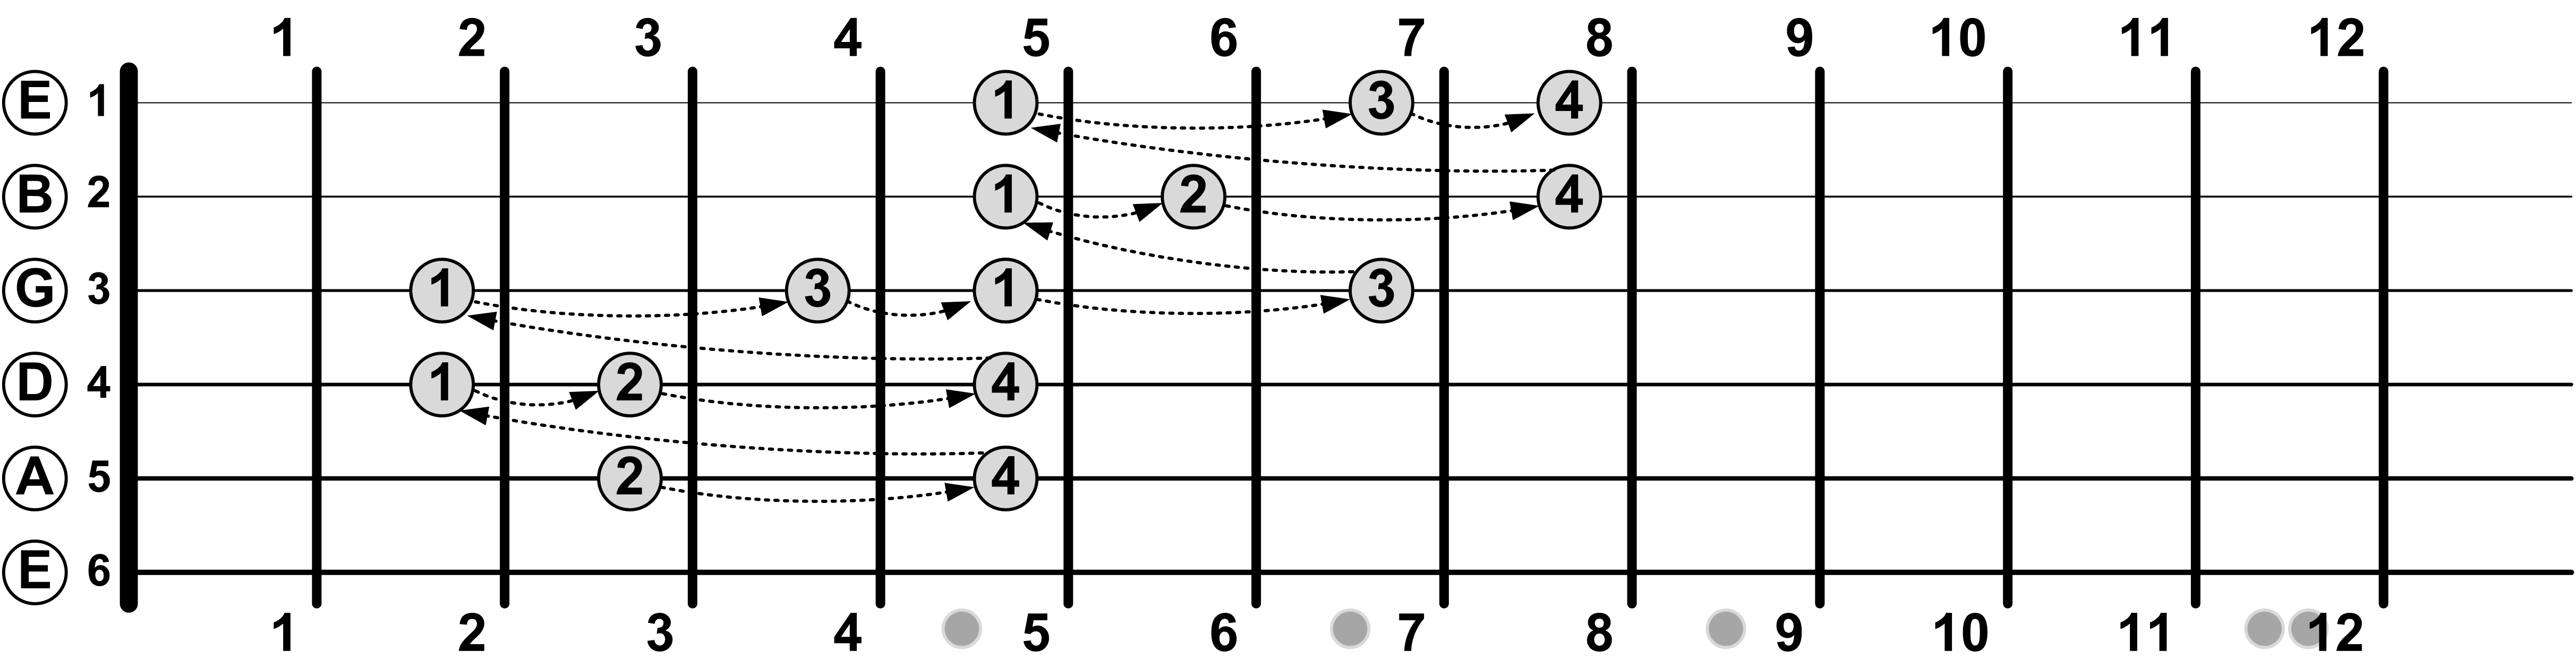
\includegraphics[width=\textwidth]{fig/intervals/c-dur-csale-segovia} 
    \caption{Аппликатура двухоктавной гаммы ДО-мажор}\label{fig:harmony:scales:c:dur:segovia}
\end{figure} 

А теперь небольшой бонус: вы научились играть не только варианты гаммы ДО-мажор. Сдвиньте, например, кисть на два лада вниз по грифу и сыграйте то, что помнят ваши руки. Вуаля: уже РЕ-мажор.



%TODO: голос? у музыки есть голос?
